\documentclass[9pt,t]{beamer}

%-------------------------------------------------
%   THEMES & PACKAGES
%-------------------------------------------------
\usetheme[progressbar=frametitle]{metropolis}
\usepackage[belowskip=-15pt]{caption}
\usepackage{graphicx}
\usepackage{subcaption}
\usepackage{wrapfig}

%-------------------------------------------------
%   Settings
%-------------------------------------------------
\setbeamertemplate{footline}[text line]{%
    \parbox{\linewidth}{\vspace*{-8pt}\insertshorttitle\hfill\insertshortsubtitle\hfill\insertshortauthor\hfill\insertpagenumber}}
\setbeamertemplate{navigation symbols}{}

%-------------------------------------------------
%   TITLE
%-------------------------------------------------
\title{Neural Networks}
\subtitle{Final Review}
\date{\today}
\author{Minh Nguyen}
\titlegraphic{\hfill
\includegraphics[height=0.7cm]{../../images/h-brs-logo.png}}

%-------------------------------------------------
%   COMMANDS
%-------------------------------------------------
\newcommand{\picEqHereWidth}[2] { %
    \begin{figure}[htp] 
        \centering
        \includegraphics[width=#2]{#1}
    \end{figure}
}
\newcommand{\picHereWidth}[4] { %
    \begin{figure}[htp] %
        \centering
        \includegraphics[width=#4]{#1} %
        \caption{#2} %
        \label{#3}
    \end{figure} %
}
%-------------------------------------------------
%   BEGIN
%-------------------------------------------------
\begin{document}

%-------------------------------------------------
\maketitle

%-------------------------------------------------
\begin{frame}{Artificial Neural Networks}
    \begin{alertblock}{ANN definition}
        \begin{itemize}
            \item massively parallel distributed processor
            \item (made up of) simple processing units
            \item (good at) storing experiential knowledge \& making it available for use
            \item resembles the brain
        \end{itemize}
    \end{alertblock}
    \begin{alertblock}{Neuron definition}
        A neuron is a \textbf{basic info processing unit of a NN}, consisting of:
        \begin{itemize}
            \item set of connecting links (\textbf{weights} or synapses)
            \item an \textbf{adder} function (linear combiner): computes weighted inputs
            \item \textbf{activation function} (squashing function): limits neuron output. Types:
            \begin{itemize}
                \item threshold (McCulloch-Pitts model): step function
                \item piece-wise linear: linear on $(\frac{-1}{2}, \frac{1}{2})$, like step function elsewhere.
                \item sigmoid.
            \end{itemize}
        \end{itemize}
    \end{alertblock}
\end{frame}

%-------------------------------------------------
\begin{frame}{Artificial Neural Networks}
    \picHereWidth{../images/neuron_graph}{Neuron graph}{fig:neuron}{0.7\linewidth}
    \begin{alertblock}{Types of NN architectures}
        \begin{itemize}
            \item single layer feed forward (neurons organized)
            \item multilayer feed forward (acyclic layers)
            \item recurrent (acyclic layers)
        \end{itemize}
    \end{alertblock}
\end{frame}

%-------------------------------------------------
\begin{frame}{Artificial Neural Networks}
    \begin{figure}[htp!]
        \centering
        \begin{subfigure}{.5\textwidth}
            \centering
            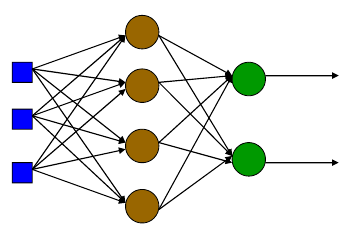
\includegraphics[width=.7\linewidth]{../images/mlp.png}
        \end{subfigure}%
        \begin{subfigure}{.5\textwidth}
            \centering
            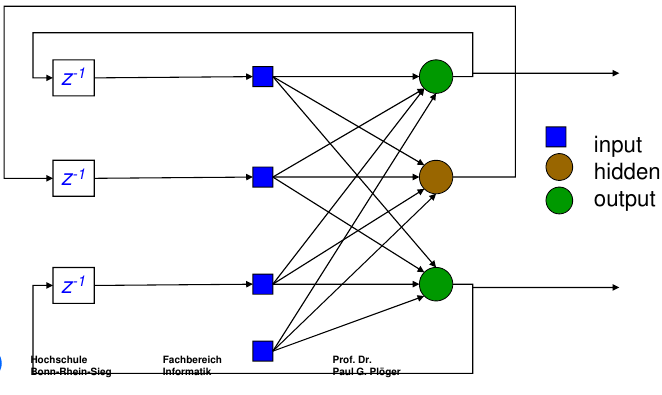
\includegraphics[width=\linewidth]{../images/rnn.png}
        \end{subfigure}
        \caption{MLP and RNN networks}
    \end{figure}
    \begin{alertblock}{Knowledge rules in ANNs}
        \begin{itemize}
            \item similar inputs from similar classes produce similar representations
            \item items from separated classes should receive different representations
            \item important features should be represented using large number of neurons
            \item prior info and \textbf{invariance} should be built-in to the network
            \begin{itemize}
                \item invariance by structure: $w_{ij} = w_{ji}$
                \item invariance by training: many examples
                \item invariant feature space
            \end{itemize}
        \end{itemize}
    \end{alertblock}
\end{frame}

%-------------------------------------------------
\begin{frame}{Artificial Neural Networks}
    \begin{wrapfigure}{r}{0.5\linewidth}
        \centering
        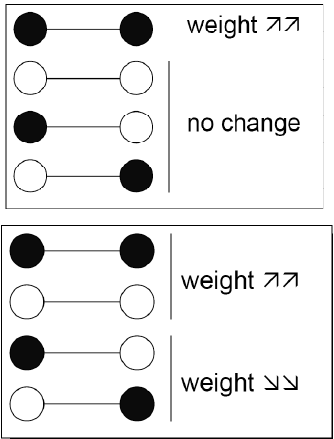
\includegraphics[width=0.8\linewidth]{../images/hebbs.png}
        \caption{Hebbs' and symmetric Hebbs' rule}
    \end{wrapfigure}
    \begin{alertblock}{Learning - Hebbs rule}
        \begin{itemize}
            \item defines how~synaptic~weights influence and are~influenced by the neurons operations
            \item weight~should~increase~when both neurons~are~excited~(black circle): increase~efficiency~of firing both neurons.
            \item symmetrical~Hebbs'~used~to avoid saturation.
        \end{itemize}
    \end{alertblock}
\end{frame}

%-------------------------------------------------
\begin{frame}{Artificial Neural Networks}
    \picHereWidth{../images/reinforce_learn.png}{Reinforcement learning}{fig:rf}{0.5\linewidth}
    \begin{alertblock}{Learning paradigms}
        \begin{itemize}
            \item supervised: build input-output relation known through examples
            \item unsupervised: model properties of inputs
            \item reinforcement learning: learn from outputs -- whether the output is good or bad.
        \end{itemize}
    \end{alertblock}
\end{frame}

%-------------------------------------------------
\begin{frame}{Artificial Neural Networks}
    \begin{alertblock}{Classification vs regression}
        \begin{itemize}
            \item regression outputs continuous values, whereas classification outputs discrete class labels
            \item regression examples: system identification, inverse modeling, controller
            \item classification examples: pattern matching,.
        \end{itemize}
    \end{alertblock}
    \begin{alertblock}{Similarity between polynomial curve fitting and NN regression}
        \begin{itemize}
            \item Similar formulation: polynoms $y = \sum_{j = 0}^{M} w_j x_j$; NN $y = f (\textbf{w}, \textbf{x})$
            \item Same error criterion $E = \sum_{p = 1}^{P}(y^p - t^p) ^2$
            \item Min error solution: polynoms -- quadratic in $\textbf{w}$, min(E) is solution of a set of linear equations; NN -- nonlinear in $\textbf{w}$, solve for local minima
        \end{itemize}
    \end{alertblock}
    \begin{alertblock}{Learning vs. generalization}
        \begin{itemize}
            \item Learning: find parameters $\textbf{w}$ to minimize error $ E $ given a set of examples
            \item Generalization: assign output value $ y $ to a new input $ x $ given $ \textbf{w} $
        \end{itemize}
    \end{alertblock}
\end{frame}

%-------------------------------------------------
\begin{frame}{Artificial Neural Networks}
    \begin{alertblock}{Overfitting}
        NN are \textbf{universal approximation models} with (relatively) \textbf{low complexity} $ \Rightarrow $ prone to overfitting
    \end{alertblock}
    \begin{alertblock}{model complexity}
        \begin{itemize}
            \item hard to compromise between performance and complexity $ \Rightarrow  $ control \emph{effective} complexity, use new error $ \tilde{E} = E + \lambda \Omega $ with penalty term:
            \[ \Omega = \frac{1}{2} \int \left(\frac{d^2 y}{x^2}\right)^2 dx \]
            \item many possible forms of $ \Omega $ and $ \lambda $ is hard to adjust.
        \end{itemize}
    \end{alertblock}
    \begin{alertblock}{Curse of dimensionality}
        \begin{itemize}
            \item More features lead to worse performance
            \item For few data samples dimension should be low
        \end{itemize}
    \end{alertblock}
\end{frame}
%-------------------------------------------------
%   END
%-------------------------------------------------
\end{document}
